%%%%%%%%%%%%%%%%%%%%%%%%%%%%%%%%%%%%%%%%%%%%%%%%%%%%%%%%%%%%%%%%
%%%%%%%%%%%  Example usage of sjsuthesis.cls %%%%%%%%%%%%%%%%%%%
%%%%%%%%%%%%%%%%%%%%%%%%%%%%%%%%%%%%%%%%%%%%%%%%%%%%%%%%%%%%%%%%

\documentclass[modernstyle,12pt]{sjsuthesis}


%%%%%%%%%%%%%%%%%%%%%%%%%%%%%%%%%%%%%%%%%%%%%%%%%%%%%%%%%%%%%%%%
%%%%%%%%%%%    load any packages which are needed    %%%%%%%%%%%
%%%%%%%%%%%%%%%%%%%%%%%%%%%%%%%%%%%%%%%%%%%%%%%%%%%%%%%%%%%%%%%%

% these are typical

\usepackage{latexsym}		% to get LASY symbols
\usepackage{epsfig}		% to insert PostScript figures
\usepackage{graphicx}           % to insert any other kind of figure

% these are for math stuff

\usepackage{amsmath}	% AMS math features (e.g., eqn alignment)
\usepackage{amssymb}	% Various weird symbols
\usepackage{amsfonts}	% Various useful math fonts
\usepackage{amsthm}	% Fancy theorem-type environments

% Convention: everything (except pictures) is numbered inside a single
% sequence, starting again in each section.  This makes things much
% easier to read.

\newtheorem{thm}{Theorem}[section]
\newtheorem{lem}[thm]{Lemma}
\newtheorem{cor}[thm]{Corollary}
\newtheorem{conj}[thm]{Conjecture}
\newtheorem*{main}{Main Theorem}
\theoremstyle{definition}
\newtheorem{defn}[thm]{Definition}
\newtheorem{rem}[thm]{Remark}
\newtheorem{exmp}[thm]{Example}
\newtheorem{ques}[thm]{Question}


%%%%%%%%%%%%%%%%%%%%%%%%%%%%%%%%%%%%%%%%%%%%%%%%%%%%%%%%%%%%%%%%
%%%%%%%%%%%%       all the preamble material:       %%%%%%%%%%%%
%%%%%%%%%%%%%%%%%%%%%%%%%%%%%%%%%%%%%%%%%%%%%%%%%%%%%%%%%%%%%%%%

\title{A Question Answering System on SQuAD Dataset Using an End-to-end Neural Network}

\author{BO}{LI}

\degree{Master of Science}		%  #1 {long descr.}
	{M.S., Computer Science}		%  #2 {short descr.}

\degreemonth{May}
\degreeyear{2018}

\dept{Department of}			%  #1 {designation}
     {Computer Science}		        %  #2 {name}

\advisor{Dr.}				%  #1 {title}
	{Chris Pollett}			%  #2 {name}
\advisorOrg{Department of Computer Science}

\reader{Dr.~Suneuy Kim}		        %  2nd person to sign thesis
\readerOrg{Department of Computer Science}

\readerThree{Dr.~David Taylor}		%  3rd person to sign thesis
\readerThreeOrg{Department of Computer Science}

% you can optionally add \readerFour and \readerFive as well

%\readerFour{Dr.~Who Dat}		%  4th person to sign thesis
%\readerFourOrg{Department of Physics, Harvard Univ.}

% NOTE: to get the front matter single spaced, put \singlespacing
% at the start of the abstract text

\abstract{Question Answering(QA) is about making a computer program that could answer questions in natural language automatically. QA techniques are widely used. End-to-end neural network architectures are state-of-art techniques for question answering tasks. Challenges of applying end-to-end models include getting more accurate results, reducing network size, explaining how the model works and so on. In this project, I focus on reducing network size and explaining the model. Based on match-lstm and answer pointer model, I design a baseline architecture. Then I make three changes to the baseline architecture to do comparisons. I successfully implemented the four models and got reasonable training and testing results. Through comparing the results of three changed models with the baseline model, I also found some redundant design in the baseline model - preprocessing layer and the $h_r$ in bidirecional match-lstm layer provides duplicate context information.
}



% acknowledgements page is optional

\acknowledgements{

Thanks to
}

% the following options can be enabled or disabled

%\ToCisShort	% a 1-page Table of Contents

% Default: List of figures will be printed
% Uncomment the \emptyLoF line to skip the list of figures
%\LoFisShort	% a 1-page List of Figures
%\emptyLoF	% no List of Figures at all

%\LoTisShort	% a 1-page List of Tables
% \emptyLoT	% no List of Tables at all


%%%%%%%%%%%%%%%%%%%%%%%%%%%%%%%%%%%%%%%%%%%%%%%%%%%%%%%%%%%%%%%%%
%%%%%%%%%%%%%%%       BEGIN DOCUMENT...         %%%%%%%%%%%%%%%%%
%%%%%%%%%%%%%%%%%%%%%%%%%%%%%%%%%%%%%%%%%%%%%%%%%%%%%%%%%%%%%%%%%

% the \begin{document} will generate all the prologue material
% (signature page, TOC, etc.); if you want to control this
% behavior, uncomment one of the following lines:
%
% \SuspendPrologue    % disables the prologue entirely
% \SimplePrologue     % prints only title, abstract, TOC, TOF


% the following command will cause a draft version and the
% current date to be printed in the header area
%
% \draftVersion{1}


\begin{document}

\raggedright          % as per SJSU GS&R guidelines June 2010
\parindent=30pt       % restores indentation

% \singlespacing      % uncomment to print single spaced (e.g., for drafts)


% document body goes here

\chapter{Introduction}

Question Answering(QA) is about making a computer program that could answer questions in natural language automatically. QA techniques are widely used among search engines, personal assistant applications on smart phones, voice control systems and a lot more other applications. In recent years, more end-to-end neural network architectures are built to do question answering tasks. The end-to-end neural network approach gives more accurate result than traditional solutions, which use syntactic and semantic analyses and hand made features.Challenges of applying end-to-end models include getting more accurate results, reducing network size, explaining how the model works and so on.

The Stanford Question Answering Dataset (SQuAD) is used in this project. As described by \cite{rajpurkar2016squad}, it includes questions asked by human beings on Wikipedia articles. The answer to each question is a segment of the corresponding Wikipedia article. In total, SQuAD contains 100,000+ question-answer pairs on 500+ articles. The goal of this project is to build a QA system on SQuAD using an end-to-end neural network architecture.

In this project, I focus on reducing network size and explaining the model. Based on match-lstm and answer pointer model designed in \cite{wang2016machine}, I design a baseline architecture. Then I make three changes to the baseline architecture to do comparisons. I successfully implemented the four models and got reasonable training and testing results. Through comparing the results of three changed models with the baseline model, I also found some redundant design in the baseline model - preprocessing layer and the $h_r$ in bidirecional match-lstm layer provides duplicate context information.



\chapter{Background}
\section{Word Feature Vector}
Word Feature Vector (WFC) was firstly came up with in \cite{bengio2003neural}. A word feature vector carries information about the likeliness of each word from the vocabulary to be its neighbour. A word feature represents a word according to its relationship with all words in the vocabulary.

\begin{figure}[htbp]\centering
  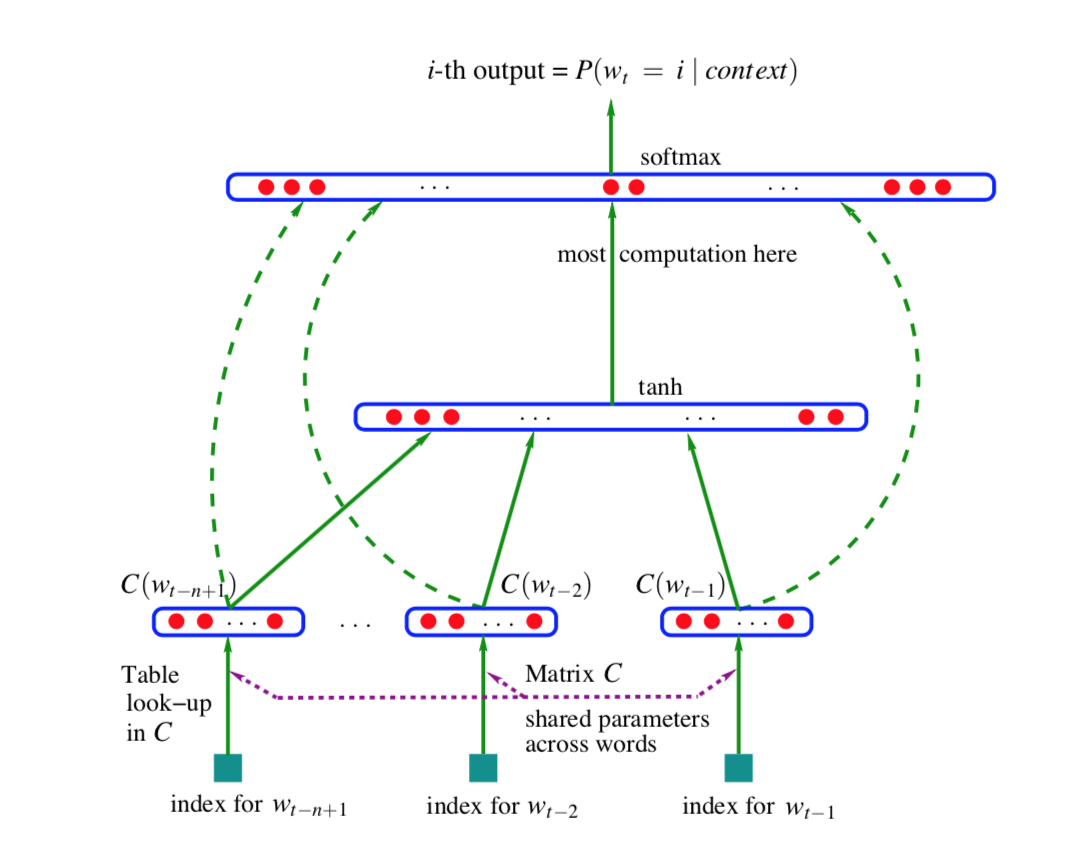
\includegraphics[width=15cm, height=12cm]{figures/nplm_architecture.png}
  \caption{Neural architecture: $f(i,w_{t-1},... ,w_{t-n+1}) =g(i,C(w_{t-1}),... ,C(w_{t-n+1}))$ where $g$ is the neural network and $C(i)$ is the $i$-th word feature vector\cite{bengio2003neural}}
  \label{f:nplm_architecture.png}
\end{figure}

As showed in Figure \ref{f:nplm_architecture.png}, the word feature vectors of a given text is learned from training a neural probabilistic language model(NPLM) on the text. The NPLM is illustrated in CITEfigurenlpmfromcs297report, where V is the vocabulary, $w_t$ represents a word from $V$, and the matrix $C$ contains the word feature vectors of all words in $V$. Each instance of the training set is a sequence of words $w_1,...,w_T$. The purpose of NPLM is to train a model $f$ such that $ f(w_t, ..., w_{t-n+1}) = \hat{P}(w_t | w_{t-1},...,w_{t-n+1})$. The computation of $f(w_t, ..., w_{t-n+1})$ is divided into two parts.
First, we map each $w$ to a WFC by selecting the corresponding row in $C$ to get $x=(C(w_{t-1}),... ,C(w_{t-n+1}))$. Second, we get $f(w_t, ..., w_{t-n+1})$ through $y=b+W\cdot x + U\cdot tanh(d + H\cdot x)$ and $ f(w_t, ..., w_{t-n+1}) = \frac{e^{y_{w_t}}}{\sum_{i}^{}e^{y_i}}$. The loss function to minimize is $L = -\frac{1}{T}\sum _{t}^{} \log{f(w_t, ..., w_{t-n+1})}$.


WFC enables learning dependencies on longer sentences. In comparison, n-grams only considers around 3 words in practice due to the computation infeasibility when n is larger. As such, a natural language model built on WFC can consider more context information than that built on n-grams. More context generally brings more more accurate result.

The usage of WFC is far beyond simply predicting a word's neighbours. In practice, WFC is a common way to represent the words in an end-to-end neural network model which does a natural language processing task.

\section{Recurrent Neural Networks (RNNs)}\label{sect:rnn}
Recurrent neural networks (RNNs) \cite{rumelhart1986learning} are neural networks with sequence-based specialization. They are used for modeling sequential data. Figure \ref{f:rnnWithNoOutputs} is a simple recurrent network with no outputs. $x$ is the input. $h$ is the hidden state. The relation between $h$ and $x$ is $h_t = f(h_{t-1}, x; \theta)$ where $\theta$ is hyperparameters.

\begin{figure}[htbp]\centering
  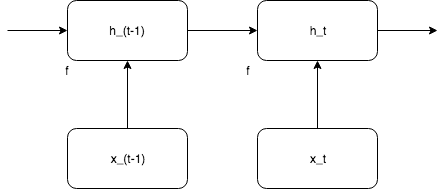
\includegraphics[width=12cm, height=3cm]{figures/rnnWithNoOutputs}
  \caption{A recurrent network with no outputs\cite{bengio2003neural}}
  \label{f:rnnWithNoOutputs}
\end{figure}

In this research, I use two types of design patterns. The first type is a RNN with recurrent connections between hidden states and the sequence of hidden states are the output of the RNN. The second type is also a RNN with recurrent connections between hidden states, but the last hidden state is the output of the RNN.

I use Long Short Term Memory (LSTM) cell and Gated Recurrent Unit (GRU) cell instead of the basic RNN cell. They prevent the RNNs from vanishing after a few iterations.

\section{Bidirectional RNNs}

The RNNs of Section \ref{sect:rnn}
iterate from left to right. As such, the $h_t$ only contains context information from $x_1$ to $x_t$, but does not contain context information from $x_{t+1}$ to the end. However, in most sequence-to-sequence tasks, we want $h_t$ to contain the information of the whole sequence. Bidirectional RNNs make this possible. In a bidirectional RNN, one RNN rolls from left to right, and another RNN rolls from right to left. As illustrated in Figure \ref{f:bidirectionalRnn}, at time t, using both $h_t$ and $g_t$ would get context information from the whole sequence.

\begin{figure}[htbp]\centering
  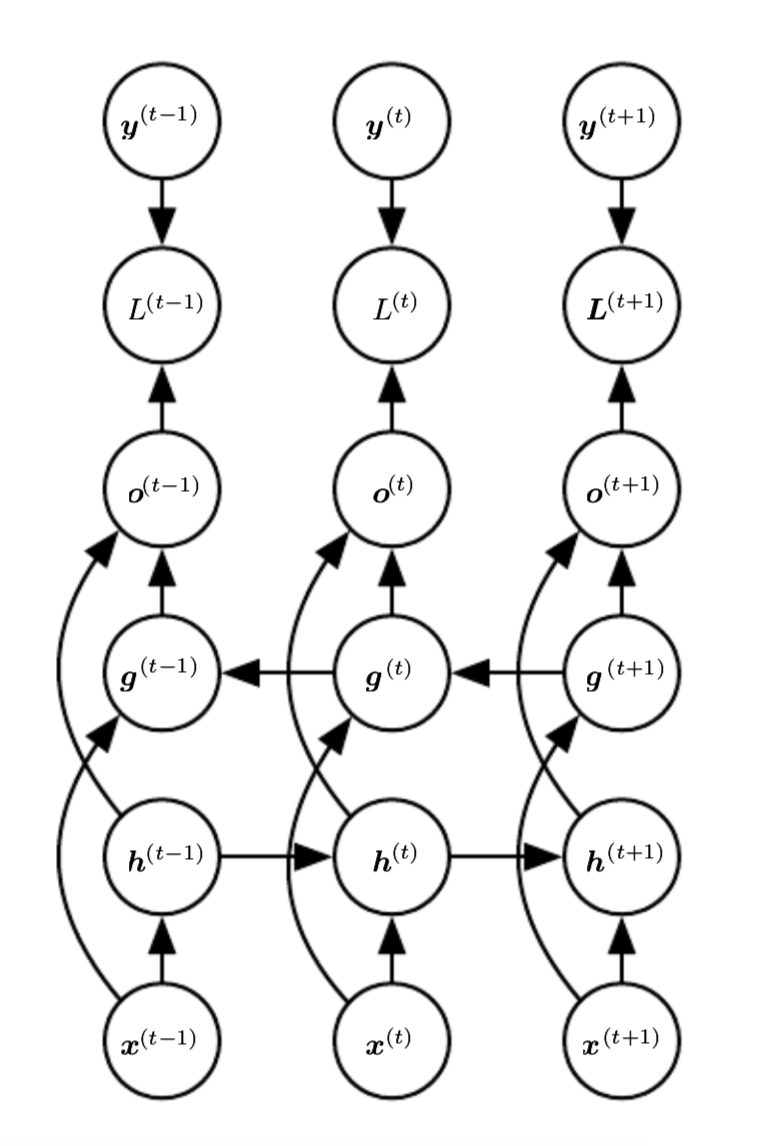
\includegraphics[width=7cm, height=10cm]{figures/bidirectionalRnn}
  \caption{A typical bidirectional recurrent neural network. $h$ and $g$ are states. $x$ is input, $o$ is output, $y$ is ground truth, $L$ is loss.\cite{goodfellow2016deep}}
  \label{f:bidirectionalRnn}
\end{figure}

\section{Encoder-Decoder Sequence-to-Sequence Architecture}

Sequence-to-sequence means the input to the model is a sequence, and the output from the model is also a sequence. An encoder-decoder architecture can be applied to do this task. The process of understanding the input sequence is considered as encoding the input sequence to some vectors $C$. The process of generating output is considered as decoding the vectors $C$.

Figure \ref{f:encoderDecoder} shows an basic encoder-decoder architecture used by some natural language processing tasks such as Machine translation and speech recongnition. The $x$s are inputs, and the $y$s are outputs.

\begin{figure}[htbp]\centering
  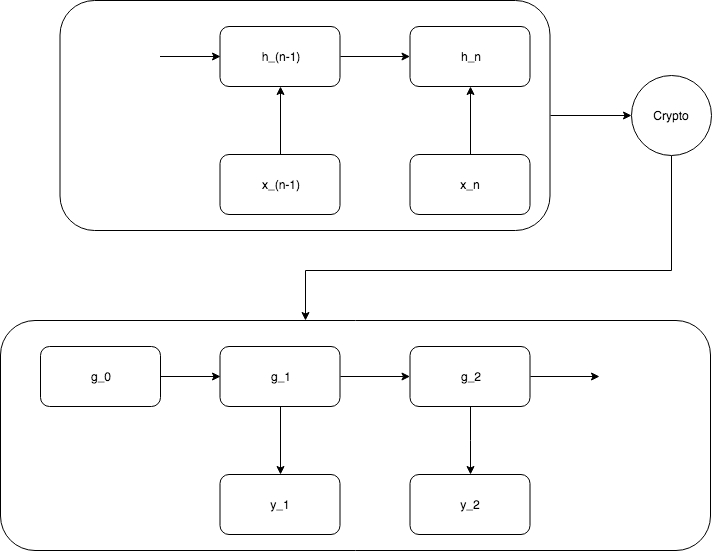
\includegraphics[width=10cm, height=10cm]{figures/encoderDecoder.png}
  \caption{An example of encoder-decoder sequence to sequence architecture\cite{goodfellow2016deep}}
  \label{f:encoderDecoder}
\end{figure}

The answer questioning task is a sequence-to-sequence task. However, the input sequences are actually two sequences - questions and passages, and the output sequences are answers. As such, in the encoding process, we need some method to make the passages aware of the questions, and encode passages and questions together to some vectors $C$. I will talk about the details in Chapter \ref{chap:design}.

\section{Attention Mechanism}\label{sect:attention}

Attention mechanism was first came up with in \cite{bahdanau2014neural} in the application of neural machine translation. Neural machine translation is also a sequence-to-sequence task. The input sequence is some words in one language, and the output sequence is the same content in another language. In the encoder-decoder sequence-to-sequence architecture for neural machine translation, a RNN encodes the input sequence to one state, and the decoder decodes the state to the output sequence. However, a big problem here is the state cannot contain all the information of a long input sequence. The attention mechanism was invented to let the decoding process knows about the input sequence.

Figure \ref{f:attention} shows how attention mechanism is added to the basic encoder-decoder architecture for machine translation described in Figure \ref{f:encoderDecoder}. When decoding $y_t$, use $s_{t-1}$ to query states of encoding process to get weights $\alpha _1 ... \alpha _T$, then get weighted average of $h_1 ... h_T$ - $c_t$, then get $s_t =f(s_{t-1},y_{t-1},c_t)$, and at last get $y_t$ from $s_t$.

\begin{figure}[htbp]\centering
  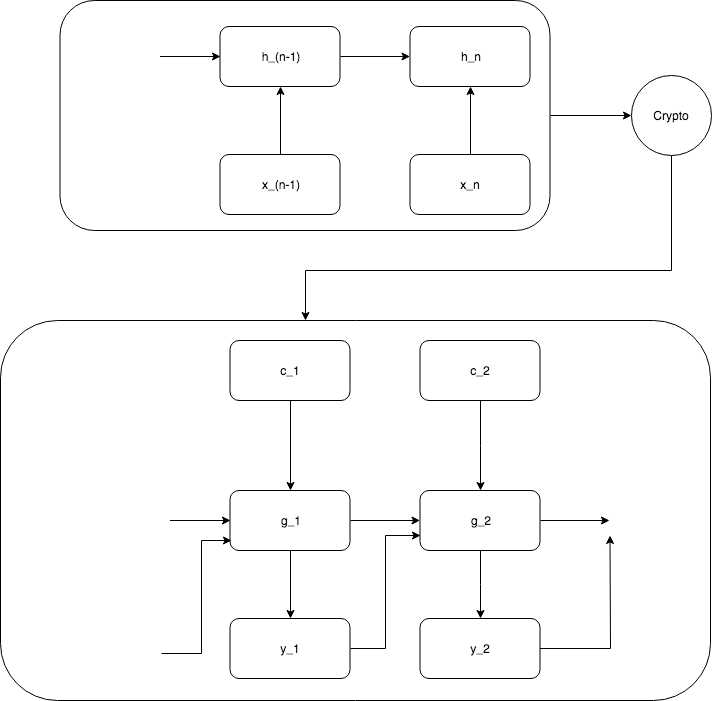
\includegraphics[width=8cm, height=10cm]{figures/attention}
  \caption{How attention is used to generate the $y_t$ \cite{bahdanau2014neural}}
  \label{f:attention}
\end{figure}

\cite{goodfellow2016deep} summarizes the attention mechanism used in neural machine translation into three components:
\begin{itemize}
\item{A process that reads raw data.}
\item{A list of feature vectors storing the output of the reader.}
\item{A process that exploits the content of the memory to sequentially perform a task, at each time step having the ability put attention on the content of one memory element (or a few, with a different weight).}
\end{itemize}



Although the attention mechanism was invented for doing machine translation task, it can be applied to many other tasks of natural language processing. I will explain how attention mechanism is used in this project in Chapter \ref{chap:design}




\section{Pointer Network}\label{sect:pointerNet}

Pointer Network\cite{vinyals2015pointer} was discovered in 2015. Pointer Network enables decoder to output a sequence of indexes in input sequence. It uses attention weight as a probability distribution to select a member from the input sequence as the output token. Taking the notation in Section \ref{sect:attention}, the output is $y_t = argmax_t{(\alpha _1 ... \alpha _T)}$. The iteration of decoding process is $s_t =f(s_{t-1},c_t)$.




\chapter{Design}\label{chap:design}

Considering the limited computation resource, I choose \cite{wang2016machine} as the main reference of my design. The model in \cite{wang2016machine} reflects a general architecture to do question answering task, and the number of layers is not too many to train. In this chapter, I introduce \cite{wang2016machine} first. Then I describe how I modify it to design my baseline architecture and how I modify the baseline architecture to analyze how the baseline architecture works.


\section{Match-lstm and Answer Pointer Model}

Wang and Jiang  proposed an encoder-decoder sequence-to-sequence architecture for the question answering task on SQuAD dataset in \cite{wang2016machine}. Each instance of training data includes one passage, one question and one answer. The passage is a sequence of tokens, the question is a sequence of tokens, and the answer is two indices indicating the start and end position in passage. Recall that each answer is part of the corresponding passage in SQuAD dataset.

Before feeding training data into model, tokens in passages and questions are vectorized to word feature vectors. As such, some pre-trained word feature vector matrix is an additional dataset in need.

The vectorized training data is feed into the encoder. The encoder includes two layers - preprocessing layer and bi-directional match-LSTM layer. In preprossing layer, a LSTM network runs over each passage word feature vector sequence and outputs a sequence of LSTM hidden states. The same LSTM is used to encode each question word vector sequence to a sequence of LSTM hidden states.

$$H^p = \overrightarrow{LSTM}(P)$$
$$H^q = \overrightarrow{LSTM}(Q)$$

where

 $$P\in R^{d \times p}: passage$$
 $$Q\in R^{d \times q}: question$$
 $$H^p\in R^{l \times p}: encoded\ passage$$
 $$H^q\in R^{l \times q}: encoded\ question$$
 $$p: length \ of\ passage$$
 $$q: length\ of\ question$$
 $$l: dimension\ of\ LSTM\ hidden\ states$$
 $$d: dimension\ of\ word\ feature\ vector$$

In bi-directional match-LSTM layer, a LSTM equipped with passage-question attention, which is called match-LSTM, is used to encode each sequence passage hidden states and the pairing sequence of question hidden states together to a sequence of hidden states of the match-LSTM. To be specific,

$$\overrightarrow{G} = tanh(W^qH^q + (W^p{h_i}^p + W^r\overrightarrow{{h_{i-1}}^r} + b^p) \otimes e_q)$$
$$\overrightarrow{\alpha _i} = softmax(w^t\overrightarrow{G_i} + b \otimes e_q)$$


where

$$W^q, W^p, W^r\in R^{l \times l} $$
$$b_p, w\in R^{l}  $$
$$b \in R $$
$$\overrightarrow{{h_{i-1}}^r}\in R^{l}: one\ column\ of\ H_p  $$

and

\[ \overrightarrow{z_i} =
\begin{bmatrix}
{h_i}^p \\
H^q\overrightarrow{ {\alpha _i}}^T \\
\end{bmatrix}
\in R^{2l}
\]
$$\overrightarrow{{h_i}^r} = \overrightarrow{LSTM}(\overrightarrow{z_i}, \overrightarrow{{h_{i-1}}^r}).$$

After iterating between getting attention vector $\overrightarrow{\alpha _i}$ and getting hidden state ${{h_{i}}^r}$ $p$ times, we get $[{{h_{1}}^r}, ..., {{h_{p}}^r}]$. Concatenate them to get

$$\overrightarrow{H_r} = [{{h_{1}}^r}, ..., {{h_{p}}^r}] \in R^{l \times p}.$$

Then go over $H_p$ from right to left to get $\overleftarrow{H_r}$. Concatenate $\overrightarrow{H_r}$ and $\overleftarrow{H_r}$ to get the final output of encoding process

\[ H_r =
\begin{bmatrix}
\overrightarrow{H_r} \\
\overleftarrow{H_r} \\
\end{bmatrix}
\in R^{2l \times p}.
\]

The decoding process includes only one layer - Answer Pointer layer. This layer is motivated by the Pointer Net in \cite{vinyals2015pointer} I have discussed in Section \ref{sect:pointerNet}. Wang and Jiang proposed two ways to design this layer. Here I only explain the boundary way. In this way, each instance of the output of the decoding process is two probability distributions. The first probability tells how likely each token in passage to be the start of the answer. The second probability distribution tells how likely each token in passage to be the end of the answer. To be specific,

$$F_k = tahn(VH_r + (W^a{h^a_{k-1}} +  b^a) \otimes e_p)$$
$$\beta _k = softmax(v^tF_k + c \otimes e_p)$$


where
$$V \in R^{l \times 2l}$$
$$W^a\in R^{l \times l} $$
$$b_a, v\in R^{l}  $$
$$c \in R $$
$${h_{k-1}}^a\in R^{l}: hidden\ state\ at\ positiom\ i\ of\ answer\ LSTM  $$

and answer LSTM is


$${h_k}^a = LSTM(H^r\beta _k^T, h_{k-1}^a)$$

By iterating between the attention mechanism and the answer LSTM two times, we could get the output of the decoding process - $\beta _0$ and $\beta _1$.


Then we can get the loss function. Let $a_s$ denote the ground truth start index of the answer, and $a_e$ denote the ground truth end index, then we have

$$p(a|H^r) = p(a_s|H_r)p(a_r|H_r)=\beta _{0, a_s} \times \beta_{1, a_e}$$

where $$\beta_{k, j} = jth\ token\ of\ \beta _k$$

To train the model, the loss function

$$J(\theta) = -\frac{1}{N}\sum_{i=1}^{N} \log{p(a^n|H^r)} $$

is minimized.

\section{Baseline Architecture}

The difference from my baseline architecture to Wang's design is the decoding part. My output of the decoding part is same with theirs, but I choose a simplified way to get there. I use the same way to get $F_k$ and $\beta _k$, but let ${h_k}^a = H^r\beta _{k}^T$ and $h_{-1}^a = \overrightarrow{0}$.

\section{First Change to Baseline Architecture}

My first change to baseline architecture is removing the $W^r\overrightarrow{{h_{i-1}}^r}$ in bi-directional match-LSTM layer. I am interested in this experiments since I guess the $\overrightarrow{{h_{i-1}}^r}$ only carries some redundant information. After this change,


$$\overrightarrow{G} = tanh(W^qH^q + (W^p{h_i}^p + b^p) \otimes e_q)$$


\section{Second Change to Baseline Architecture}

My second change to baseline architecture is removing the preprocessing layer in encoding process.

\section{Third Change to Baseline Architecture}

My third change is combining the first and second change.

\chapter{Implementation}

\section{Padding}\label{sect:padding}

In practice, passages have different length, and questions also have different length. We must cut or extend all passages to a same length, and all questions to a same length. This process is called padding. Due to padding, the architecture in implementation has some difference with the theoretical one.

Assume in data processing step, each passage is paired with one $passage_mask$ vector of size $passage_padding_length$, and each question is paired with one $question_mask$ of size $question_padding_length$. The entry of mask vector is either 0 or 1. 0 indicates the current token does not exit in original sequence.

In preprocessing layer,
$$H^p = H^p \circ (passage\_mask \otimes l)$$
$$H^q = H^q \circ (question\_mask \otimes l)$$

In match-LSTM layer,
$$\overrightarrow{\alpha _i} = softmax( (w^t\overrightarrow{G_i} + b \otimes e_q) ) \circ question\_mask $$


$$H_r = H_r \circ (passage\_mask \otimes 2l)$$

In Ans-Ptr layer,
$$\beta _k = softmax( (v^tF_k + c \otimes e_p) ) \circ passage\_mask$$


\section{Tensorflow Graph}
I use Tensorflow to do implementation. Tensorflow is an open source machine learning framework. The central idea of Tensorflow is describing a complex numeric computation as a graph. Each node of a graph is a operation, and the edges of a node are values needed to perform the operation. Variables are "trainable" nodes. Placeholders are nodes whose values are fed in run time. Take the baseline architecture as example, variables should be used to represent all the parameters of encoding and decoding layers, and placeholders should be used to represent passages, questions, and answers.

To train a graph, we do not need to compute the gradients on our own. Instead, we call some APIs of Tensorflow to get a train operation, and then feed data through placeholders to the operation to update the parameters.



Figure CITE describes the graph for baseline architecture. To convey information clearly, some nodes describe subgraphs instead of the original nodes. TODOdescribethefigure

TODO:conceptionalFigureOfTfGraphOfBaseline




\section{Implementation Pipelines}

TODO:figureOfWholePipeline

\chapter{Experiments}
\section{Data}
I use Stanford Question Answering Dataset (SQuAD) to do experiemnts.  It contains 100,000+ question-answer pairs on 500+ articles. The training set and dev set are visible to users. However, the test set is hidden. To perform my experiments, I split the training set into my training and dev set, and use the dev set as my test set. After such splitting, my training set contains 78839 question-answer pairs, my dev set contains 8760 question-answer pairs, and my test set contains 10570 question-answer pairs.

 Regarding to data processing, I use a Python natural language processing library {\tt nltk} to tokenize raw strings in json file into passage-question-answer triplets in the format of word token sequences.

Then I face two ways to represent the word tokens. The first way is to query the corresponding word vector of each token from the GloVe embedding matrix and turn the word sequences into vector sequences.  The second way is to make a vocabulary and turn each word sequence to an index sequence based on the vocabulary. At the same time, a smaller embedding matrix is made from the original GloVe embedding matrix. The index of each token in this matrix is same with that in vocabulary. The index sequences and the smaller embedding matrix is fed into the neural network. Since the index sequences require much less memory than the vector sequences, the second way saves a lot of memory than the first way when large data set is used.

The next step is to pad passage and question, as mentioned in Section \ref{sect:padding}. There is a {\tt pad} token in vocabulary, and the corresponding word vector is zero vector.

At last, split data into batches.

After training, the embedding matrix becomes part of the tensorflow graph, and is unchanged during testing. Also, the vocabulary remains unchanged during testing. Words not found in vocabulary during testing are treated as unknown word. The word vector of unknown words is the average of all vectors of known words in my training and dev set.

TODO: table: size of train, dev and test set

TODO: table: size of json file, voc file, embedding matrix file, token\_id file of train and valid data

TODO: figure: work flow of data processing

\section{Settings}
At the first step, I refer to the experimental settings in InnerPeace-Wu's Github page to set some of my parameters. The dimension of GloVe word vectors is 100, the size of hidden units is 64, the regularization scale of L2-regularization is 0.001 and the batch size is 32. For passage length and question length, I plot out their distributions and find out that 400 is a reasonable cut point for passage, and 30 is a reasonable cut point for question.

TODO: figure of passage length, question length

I use the default settings of tensorflow for adam optimizer. I sample out 200 instances from train set to estimate train error, and from dev set to estimate validation error. The normalization boundary to clip gradients is set as 5.

Then I do several experiments on different learning rate, since this is the most important parameters. I initially planed to do this on the match architecture, but due to some code bugs at that time, I actually do the experiments on match\_change1 architecture. I started the experiments from 0.002, which is used in InnerPeace-Wu's Github page. It performs well. Then I try several larger value. However, all the larger values I try do not perform well. So I set learning rate to 0.002.

TODO: figure of different lr


The settings that work well on one architectures also work well on other three architectures. This really sames a lot of time and money.

I used Tesla K80 12 GB Memory 61 GB RAM 100 GB SSD GPU to train the four models.

TODO: table of all experimental settings

I use F1 score and exact match score to evaluate the performance of each architecture. TODO:explain F1 and em


\section{Results}

For match architecture, the model converges after around 8 epochs. Match\_change1 and match\_change2 perform similar to match. For match\_change2, the model converges after around 4 epochs.  including training time, loss change, score change etc. For all four architectures, training each epoch costs around 2 hours on the Tesla GPU I use.

TODO:figureoftrainingstat

Figure TODO:citefigure shows the testing results of on test data set of the four architectures. In the original dev set, which is our test set, each question corresponds to multiple answers. This makes sense since in reality we might have several different ways to answer a same question. We use two ways to calculate the scores. The first way is choose the first answer, the second way is calculating scores for each answer and choose the best score.In either way, match, match\_change1 and match\_change2 perform similarly, but match\_change3 behaves much worse than the other three.


TODO:figureoftestingresult

Interactive Testing on match architecture shower some interesting reuslts.

TODO:figures of interactive testing result.

\section{Analysis}
We can draw several interesting insights from the results. First, more context information increases, or at least does not decrease the accuracy. Second, the ways to add context information are various. Third, duplicate context might not be necessary.





\chapter{Conclusion}

In this project, I developed four models for the question answering task using the Stanford Question Answering (SQuAD) dataset based on Wang's match-LSTM and Pointer Network model. I successfully implemented the four models and got reasonable training and testing results. Through comparing the results of three changed models with the baseline model, I also found some redundant design in the baseline model - preprocessing layer and the $h_r$ in bidirecional match-lstm layer provides duplicate context information.

In the future, I plan to research on the opposite direction - adding more context information to the existing model.


% if you want to keep macros or chapters in separate files
% you can do that and include them with \input like this:

%\input macros.tex
%\input ch1.tex
%\input ch2.tex


%%%%%%%%%%%%%%%%%%%%%%%%%%%%%%%%%%%%%%%%%%%%%%%%%%%%%%%%%%%%%%%%%%%
%%%%%%%%%%%%%%%%%%%%%%%  Bibliography %%%%%%%%%%%%%%%%%%%%%%%%%%%%%
%%%%%%%%%%%%%%%%%%%%%%%%%%%%%%%%%%%%%%%%%%%%%%%%%%%%%%%%%%%%%%%%%%%

\bibliographystyle{amsalpha}	% or "siam", or "alpha", or "abbrv"
				% see other styles in
				% texmf/bibtex/bst

%\nocite{*}		% uncomment to list all refs in database,
			% cited or not.

\bibliography{refs}		% assumes bib database in "refs.bib"

%%%%%%%%%%%%%%%%%%%%%%%%%%%%%%%%%%%%%%%%%%%%%%%%%%%%%%%%%%%%%%%%%%%
%%%%%%%%%%%%%%%%%%%%%%%%  Appendices %%%%%%%%%%%%%%%%%%%%%%%%%%%%%%
%%%%%%%%%%%%%%%%%%%%%%%%%%%%%%%%%%%%%%%%%%%%%%%%%%%%%%%%%%%%%%%%%%%

% \appendix	% don't forget this line if you have appendices!

% \chapter{Gratuitous Appendix}
% Nothing to see here.

% %\input appA.tex


%%%%%%%%%%%%%%%%%%%%%%%%%%%%%%%%%%%%%%%%%%%%%%%%%%%%%%%%%%%%%%%%%%%
%%%%%%%%%%%%%%%%%%%%%%%%   THE END   %%%%%%%%%%%%%%%%%%%%%%%%%%%%%%
%%%%%%%%%%%%%%%%%%%%%%%%%%%%%%%%%%%%%%%%%%%%%%%%%%%%%%%%%%%%%%%%%%%

\end{document}
